\documentclass[conference]{IEEEtran}
\usepackage[utf8]{inputenc}
\usepackage[T1]{fontenc}
\usepackage[portuguese]{babel}

\usepackage{float} 
\usepackage{url}  
\usepackage{multirow}
\usepackage{caption}
\usepackage{subcaption}
\usepackage{booktabs}
\usepackage{cite}
\pagestyle{plain}
\usepackage{amsmath}
\usepackage{float}
\usepackage{tikz}
\usepackage{placeins}
\usepackage{comment}
\usepackage{tabularx}
\usepackage{algorithm}
\usepackage{algpseudocode}
\usepackage{graphicx}
\floatname{algorithm}{Algoritmo}
\ifCLASSINFOpdf
  \usepackage[pdftex]{graphicx}
\fi

\hyphenation{op-tical net-works semi-conduc-tor}

\begin{document}

%selection sort, insertion sort, quick sort(LR PTRS), merge sort, heap sort, radix sort (LSD e MSD), std sort gcc, std::stable_sort gcc, shell sort, cocktail shaker, gnome sort, bitonic sort, bogo sort
\title{algortimos de ordenacao ? referencias}

\author{\IEEEauthorblockN{\\ Hugo Veríssimo}
\IEEEauthorblockA{Optimização Combinatória 24/25\\
Universidade de Aveiro\\
Aveiro, Portugal\\
hugoverissimo@ua.pt}
\and
\IEEEauthorblockN{\\ João Cardoso}
\IEEEauthorblockA{Optimização Combinatória 24/25\\
Universidade de Aveiro\\
Aveiro, Portugal\\
joaopcardoso@ua.pt}}

\maketitle
\thispagestyle{plain}

\begin{abstract}
rever italico ou não no nome dos coisos + "sort" VS "Sort" + mathcal O VS normal math O
\end{abstract}

\begin{quote}
\small
\noindent
\textbf{Palavras-chave:} zzz, aaa
\end{quote}

\IEEEpeerreviewmaketitle

\section{Introdução}

Os algoritmos de ordenação são essenciais em várias áreas da optimização combinatória e da investigação operacional, sendo utilizados para organizar dados de forma eficiente, melhorar o desempenho de algoritmos de procura e reduzir a complexidade computacional de problemas em larga escala.

Em contextos de otimização combinatória, onde para vários problemas se torna fundamental a ordenação prévia de dados, como nas heurísticas para o problema Knapsack, no algoritmo de Kruskal para construção de árvores geradoras mínimas, ou em algoritmos gulosos para cobertura de conjuntos, a escolha do método de ordenação pode impactar significativamente a eficiência global da solução.

% POR MELHORAR ESTE PARÁGRAFO
Este trabalho visa explorar os principais algoritmos de ordenação, destacando as suas características, o seu funcionamento, a complexidade computacional associada e uma análise comparativa entre os mesmos. Considerando as diferentes implementações e constrangimentos associados, exploramos os cenários onde cada algoritmo poderá ser mais útil. 
%SERÃO ABORDADOS ALGORITMOS COMO O QUICKSORT, .........
O objetivo é compreender como a ordenação pode ser utilizada de forma estratégica para melhorar a eficiência de algoritmos em diversos cenários, e como otimizações na própria ordenação podem levar a avanços significativos em problemas computacionalmente intensivos.

% Like insertion sort, bubble sort is adaptive, which can give it an advantage over algorithms like quicksort. This means that it may outperform those algorithms in cases where the list is already mostly sorted (having a small number of inversions), despite the fact that it has worse average-case time complexity. For example, bubble sort is O ( n ) {\displaystyle O(n)} on a list that is already sorted, while quicksort would still perform its entire O ( n log ⁡ n ) {\displaystyle O(n\log n)} sorting process. Útil para discutir os resultados, e potencial utilidade

\section{Algoritmos de Ordenação}

Nesta secção serão apresentados os algoritmos selecionados, detalhando-se individualmente o seu princípio básico de funcionamento, a complexidade temporal, as vantagens e desvantagens, e a aplicabilidade prática em diferentes cenários da otimização combinatória. POR REVER SE REALMENTE SE FAZ ISTO TUDO E MUDAR ?!?!?!??!

\subsection{Bubble Sort acrescentar informação sobre a família Exchange sorts}

O algoritmo \textit{Bubble sort} consiste em comparar um dado item com todos os elementos de uma lista, em que o item vai se reposicionando com elementos comparativamente menores até encontrar um item maior ou chegar ao fim da lista. O nome do algoritmo prende-se com a forma como o elemento comparado vai ascendendo (ou afundando, consoante seja usado), tal como uma bolha na água. 

Tipicamente este algoritmo não encontra aplicação em casos reais devido à sua ineficiência e complexidade de ordem \(O(n^2)\). No entanto, a sua rápida implementação pode ser de interesse em casos particulares, em que listas que estejam próximas da sua forma ordenada passam pelo algoritmo com uma complexidade de ordem \(O(n)\).

\begin{algorithm}[H]
    \raggedright
    \vspace{.1em}
    \textbf{Entrada:} lista \textit{arr} \\
    \textbf{Saída:} lista ordenada \textit{arr} \\
    \vspace{.5em}
    \hrule 
    \caption{Bubble Sort}
    \begin{algorithmic}[1]
        \State $n \gets$ \text{len}$(arr)$
        
        \For{$i$ from $0$ to $n - 1$}
            \State $swapped \gets$ False
            \For{$j$ from $0$ to $n - 2 - i$}
                \If{$arr[j] > arr[j+1]$}
                    \State Swap $arr[j]$ and $arr[j+1]$
                    \State $swapped \gets$ True
                \EndIf
            \EndFor
            \If{not $swapped$}
                \State \textbf{break}
            \EndIf
        \EndFor
    
        \State \Return $arr$
    \end{algorithmic}
\end{algorithm}

FALAR DA COMPLEXIDADE DO ALGORITMO A PARTIR DA ANÁLISE DO MESMO + BEST AND WORST CASE

Existem algoritmos baseados nesta abordagem, tal como o \textit{Cocktail sort}, que aplica a metodologia em sentido crescente e decrescente, tornando-o mais rápido por norma, mas com o mesmo grau de complexidade no pior cenário.

\subsection{Selection Sort}

O algoritmo de \textit{Selection sort} tem um procedimento bastante diferente do algoritmo anterior. Faz parte da família de algoritmos de \textit{Selection sorts}, em que a lista de items ordenados vai sendo gerada por comparação a partir da lista original desordenada. No algoritmo em questão, procura-se o menor elemento disponível e coloca-se no início da nova lista. Estes passos repetem-se na lista desordenada até não existirem mais e a lista ordenada ser criada.

\begin{algorithm}[H]
    \raggedright
    \vspace{.1em}
    \textbf{Entrada:} lista \textit{arr} \\
    \textbf{Saída:} lista ordenada \textit{arr} \\
    \vspace{.5em}
    \hrule 
    \caption{Selection Sort}
    \begin{algorithmic}[1]
        \State $n \gets$ \text{len}$(arr)$
    
        \For{$i$ from $0$ to $n - 1$}
            \State $min\_idx \gets i$
            \For{$j$ from $i + 1$ to $n - 1$}
                \If{$arr[j] < arr[min\_idx]$}
                    \State $min\_idx \gets j$
                \EndIf
            \EndFor
            \If{$min\_idx \neq i$}
                \State Swap $arr[i]$ and $arr[min\_idx]$
            \EndIf
        \EndFor
    
        \State \Return $arr$
    \end{algorithmic}
\end{algorithm}

A complexidade do algoritmo pode ser analisada com base no número de comparações e trocas realizadas. O número de comparações é sempre o mesmo, independentemente da ordem inicial dos dados. Para uma lista com \( n \) elementos, o número total de comparações realizadas é dado por \((n-1) + (n-2) + \ldots + 1 = \frac{n(n-1)}{2}\), o que corresponde a uma complexidade de ordem \(\mathcal{O}(n^2)\) tanto no melhor como no pior caso.

O número de trocas, por outro lado, depende da configuração inicial da lista. No melhor caso, quando a lista já está ordenada, o índice do menor elemento nunca difere do índice atual, pelo que nenhuma troca é efetuada. Assim, o número de trocas é zero. No pior caso, quando a lista está em ordem inversa, cada iteração do algoritmo encontra um menor elemento que precisa de ser trocado, resultando em \(n - 1\) trocas. Neste caso, o número de trocas é linear, ou seja, de ordem \(\mathcal{O}(n)\).

Em resumo, o algoritmo Selection Sort tem complexidade temporal \(\mathcal{O}(n^2)\) em todos os casos, realiza poucas trocas (até \(n-1\)), não é adaptativo à ordenação inicial dos dados e não é um algoritmo estável.


Dentro desta família de algoritmos, há um que devemos destacar, chamado \textit{Gnome sort},  que consiste nas operações do \textit{Selection sort}, mas sem ter o segundo ciclo dentro do primeiro, resultando num número de operações semelhante ao \textit{Insertion sort}, e por consequência pior que o \textit{Selection sort}.

\subsection{Insertion Sort}

O algoritmo Insertion Sort ordena uma lista construindo progressivamente uma sublista ordenada à esquerda. A cada passo, o elemento atual é comparado com os anteriores e inserido na posição correta, deslocando os elementos maiores uma posição à frente.

\begin{algorithm}[H]
    \raggedright
    \vspace{.1em}
    \textbf{Entrada:} lista \textit{arr} \\
    \textbf{Saída:} lista ordenada \textit{arr} \\
    \vspace{.5em}
    \hrule 
    \caption{Insertion Sort}
    \begin{algorithmic}[1]
        \For{$i$ from $1$ to $\text{len}(arr) - 1$}
            \State $key \gets arr[i]$
            \State $j \gets i - 1$
            \While{$j \geq 0$ and $arr[j] > key$}
                \State $arr[j + 1] \gets arr[j]$
                \State $j \gets j - 1$
            \EndWhile
            \State $arr[j + 1] \gets key$
        \EndFor
    
        \State \Return $arr$
    \end{algorithmic}
\end{algorithm}

A complexidade do algoritmo pode ser analisada considerando o número de comparações e movimentações de elementos. No pior caso, a lista está em ordem inversa. Cada novo elemento precisa de ser comparado com todos os anteriores e movido para o início da lista. Assim, o número total de comparações e deslocações neste caso é dado por \((1 + 2 + \ldots + n-1) = \frac{n(n-1)}{2}\), o que resulta numa complexidade temporal de ordem \(\mathcal{O}(n^2)\).

No melhor caso, a lista já está ordenada. O algoritmo ainda percorre os elementos, mas como nenhuma comparação resulta em troca, cada elemento é apenas comparado uma vez. Neste cenário, o número total de comparações é linear, e a complexidade temporal é \(\mathcal{O}(n)\).

No caso médio, assume-se que metade dos elementos anteriores são maiores que o atual, levando a aproximadamente metade das comparações do pior caso, o que continua a resultar em complexidade \(\mathcal{O}(n^2)\).

Em termos de eficiência prática, o Insertion Sort é eficiente para listas pequenas ou quase ordenadas, e tem a vantagem de ser estável, além de funcionar em tempo linear no melhor caso.

Resumindo, o algoritmo apresenta complexidade:
\[
\begin{cases}
\mathcal{O}(n) & \text{melhor caso (lista ordenada)} \\
\mathcal{O}(n^2) & \text{pior caso (lista inversamente ordenada)} \\
\mathcal{O}(n^2) & \text{caso médio}
\end{cases}
\]

\subsection{Counting Sort}

O algoritmo Counting Sort é um algoritmo de ordenação não comparativo, apropriado para listas de números inteiros não negativos e com amplitude limitada. A ideia principal consiste em contar quantas vezes cada valor ocorre e depois reconstruir a lista ordenada a partir dessas contagens.

\begin{algorithm}[H]
    \raggedright
    \vspace{.1em}
    \textbf{Entrada:} lista \textit{arr} \\
    \textbf{Saída:} lista ordenada \textit{sorted\_arr} \\
    \vspace{.5em}
    \hrule 
    \caption{Counting Sort}
    \begin{algorithmic}[1]
        \State $max\_val \gets \max(arr)$
        \State $count \gets$ array of zeros with length $max\_val + 1$
        
        \For{each $num$ in $arr$}
            \State $count[num] \gets count[num] + 1$
        \EndFor
    
        \State $sorted\_arr \gets$ empty list
        \For{$i$ from $0$ to $max\_val$}
            \If{$count[i] > 0$}
                \State Append $count[i]$ copies of $i$ to $sorted\_arr$
            \EndIf
        \EndFor
    
        \State \Return $sorted\_arr$
    \end{algorithmic}
\end{algorithm}

A complexidade do algoritmo depende de dois fatores: o tamanho da lista \( n \) e o maior valor presente, denotado por \( k = \max(\text{arr}) \). A primeira parte do algoritmo percorre a lista original e preenche um vetor auxiliar \texttt{count} de tamanho \( k + 1 \), incrementando as posições correspondentes. Esta etapa tem complexidade \(\mathcal{O}(n)\). Em seguida, o algoritmo percorre o vetor \texttt{count}, que tem tamanho \( k + 1 \), e reconstrói a lista ordenada. Esta etapa tem complexidade \(\mathcal{O}(k)\).

Assim, a complexidade total do algoritmo é \(\mathcal{O}(n + k)\), tanto no melhor como no pior caso. Não há distinção entre diferentes ordens iniciais da lista, pois o algoritmo não realiza comparações entre os elementos.

O melhor desempenho é alcançado quando \( k \) é da mesma ordem de \( n \), resultando em tempo linear. No entanto, se \( k \) for muito maior que \( n \), o algoritmo torna-se ineficiente em termos de espaço e tempo, pois aloca um vetor proporcional a \( k \), independentemente de quantos desses valores realmente aparecem.

Em resumo, a complexidade do Counting Sort é:
\[
\mathcal{O}(n + k)
\]
em todos os casos, sendo eficiente apenas quando \( k \in \mathcal{O}(n) \). O algoritmo é estável e apropriado para ordenar valores inteiros com gama pequena e conhecida.

\subsection{Radix Sort}

O algoritmo Radix Sort ordena números inteiros processando-os dígito a dígito, a partir do dígito menos significativo até ao mais significativo. Em cada passo, aplica-se um algoritmo de ordenação estável, geralmente o Counting Sort, para ordenar os elementos com base no dígito atual. O número de iterações é igual ao número de dígitos do maior número presente na lista.

\begin{algorithm}[H]
    \raggedright
    \vspace{.1em}
    \textbf{Entrada:} lista \textit{arr} \\
    \textbf{Saída:} lista ordenada \textit{arr} \\
    \vspace{.5em}
    \hrule 
    \caption{Radix Sort}
    \begin{algorithmic}[1]
        \Function{CountingSortRadix}{$arr$, $exp$}
            \State $n \gets$ \text{len}$(arr)$
            \State $output \gets$ array of zeros of length $n$
            \State $count \gets$ array of zeros of length $10$
    
            \For{$i$ from $0$ to $n - 1$}
                \State $index \gets (arr[i] \div exp) \bmod 10$
                \State $count[index] \gets count[index] + 1$
            \EndFor
    
            \For{$i$ from $1$ to $9$}
                \State $count[i] \gets count[i] + count[i - 1]$
            \EndFor
    
            \For{$i$ from $n - 1$ to $0$}
                \State $index \gets (arr[i] \div exp) \bmod 10$
                \State $output[count[index] - 1] \gets arr[i]$
                \State $count[index] \gets count[index] - 1$
            \EndFor
    
            \For{$i$ from $0$ to $n - 1$}
                \State $arr[i] \gets output[i]$
            \EndFor
        \EndFunction
    
        \State $max\_num \gets \max(arr)$
        \State $exp \gets 1$
        \While{$max\_num \div exp > 0$}
            \State \Call{CountingSortRadix}{$arr$, $exp$}
            \State $exp \gets exp \times 10$
        \EndWhile
    
        \State \Return $arr$
    \end{algorithmic}
\end{algorithm}

Seja \( n \) o número de elementos da lista, \( k \) o valor máximo presente, e \( d \) o número de dígitos de \( k \) na base decimal. Em cada uma das \( d \) iterações, o Counting Sort é aplicado com complexidade \(\mathcal{O}(n + b)\), onde \( b \) é a base usada (tipicamente 10). Como \( b \) é constante, o custo de cada iteração é \(\mathcal{O}(n)\).

Assim, a complexidade total do algoritmo Radix Sort é:
\[
\mathcal{O}(d \cdot n)
\]
como \( d = \lfloor \log_{10}(k) \rfloor + 1 \), pode também escrever-se como \(\mathcal{O}(n \cdot \log k)\) para base 10. Esta complexidade mantém-se tanto no melhor como no pior caso, já que todos os elementos são sempre processados integralmente, independentemente da ordem inicial.

O Radix Sort é eficiente quando os números têm número limitado de dígitos (isto é, \( d \in \mathcal{O}(1) \)), caso em que o tempo de execução é linear em \( n \). No entanto, o algoritmo não é comparativo e apenas funciona diretamente para inteiros ou representações discretizáveis. Além disso, o consumo de espaço extra é \(\mathcal{O}(n + b)\) por iteração.

Em resumo, o algoritmo apresenta complexidade:
\[
\mathcal{O}(n \cdot d) = \mathcal{O}(n \cdot \log k)
\]
em todos os casos, e é estável, não comparativo e adequado para listas grandes de inteiros com número de dígitos moderado.


\subsection{Quick Sort}

O algoritmo Quick Sort é um algoritmo de ordenação baseado no paradigma de dividir-para-conquistar. Escolhe um elemento como pivô e reorganiza a lista de forma que todos os elementos menores ou iguais ao pivô fiquem à esquerda, e os maiores à direita. Em seguida, aplica-se recursivamente o mesmo procedimento às duas sublistas geradas.

\begin{algorithm}[H]
    \raggedright
    \vspace{.1em}
    \textbf{Entrada:} lista \textit{arr} \\
    \textbf{Saída:} lista ordenada \textit{arr} \\
    \vspace{.5em}
    \hrule 
    \caption{Quick Sort}
    \begin{algorithmic}[1]
        \Function{Partition}{$items$, $low$, $high$}
            \State $pivot \gets items[high]$
            \State $i \gets low - 1$
            \For{$j$ from $low$ to $high - 1$}
                \If{$items[j] \leq pivot$}
                    \State $i \gets i + 1$
                    \State Swap $items[i]$ and $items[j]$
                \EndIf
            \EndFor
            \State Swap $items[i + 1]$ and $items[high]$
            \State \Return $i + 1$
        \EndFunction
    
        \Function{QuickSort}{$items$, $low$, $high$}
            \If{$low < high$}
                \State $pivot\_index \gets$ \Call{Partition}{$items$, $low$, $high$}
                \State \Call{QuickSort}{$items$, $low$, $pivot\_index - 1$}
                \State \Call{QuickSort}{$items$, $pivot\_index + 1$, $high$}
            \EndIf
        \EndFunction
    
        \State \Call{QuickSort}{$arr$, $0$, $\text{len}(arr) - 1$}
        \State \Return $arr$
    \end{algorithmic}
\end{algorithm}

A complexidade do algoritmo depende da qualidade da escolha do pivô em cada chamada recursiva. No melhor caso, o pivô divide o array em duas partes aproximadamente iguais a cada etapa. A profundidade da recursão será então \(\log n\), e em cada nível realiza-se um número total de operações proporcional a \(n\), resultando numa complexidade total de:
\[
\mathcal{O}(n \log n)
\]

No pior caso, o pivô escolhido é sempre o menor ou o maior elemento, fazendo com que uma das sublistas tenha tamanho zero e a outra contenha \(n - 1\) elementos. O número de chamadas recursivas será então \(n\), e o número total de comparações será da ordem de:
\[
\mathcal{O}(n^2)
\]

O caso médio, assumindo uma escolha aleatória ou razoável do pivô, também resulta em complexidade esperada de \(\mathcal{O}(n \log n)\). É importante destacar que a versão apresentada do algoritmo não é estável e realiza ordenação in-place, com consumo de memória adicional proporcional à profundidade da pilha de chamadas recursivas (em média \(\mathcal{O}(\log n)\)).

Em resumo, a complexidade do Quick Sort é:
\[
\begin{cases}
\mathcal{O}(n \log n) & \text{melhor caso (divisões equilibradas)} \\
\mathcal{O}(n^2) & \text{pior caso (divisões altamente desequilibradas)} \\
\mathcal{O}(n \log n) & \text{caso médio (pivôs aleatórios ou bons)}
\end{cases}
\]


\subsection{Merge Sort}

O algoritmo Merge Sort é um algoritmo de ordenação baseado no paradigma de dividir-para-conquistar. A cada passo, divide recursivamente a lista ao meio até obter sublistas de tamanho 1, e depois combina essas sublistas de forma ordenada, reconstruindo a lista original em ordem crescente.

\begin{algorithm}[H]
    \raggedright
    \vspace{.1em}
    \textbf{Entrada:} lista \textit{arr} \\
    \textbf{Saída:} lista ordenada \textit{arr} \\
    \vspace{.5em}
    \hrule 
    \caption{Merge Sort}
    \begin{algorithmic}[1]
        \Function{MergeSort}{$arr$}
            \If{$\text{len}(arr) > 1$}
                \State $mid \gets \text{len}(arr) \div 2$
                \State $left \gets arr[0 : mid]$
                \State $right \gets arr[mid : ]$
                
                \State \Call{MergeSort}{$left$}
                \State \Call{MergeSort}{$right$}
    
                \State $i, j, k \gets 0, 0, 0$
                \While{$i < \text{len}(left)$ and $j < \text{len}(right)$}
                    \If{$left[i] \leq right[j]$}
                        \State $arr[k] \gets left[i]$
                        \State $i \gets i + 1$
                    \Else
                        \State $arr[k] \gets right[j]$
                        \State $j \gets j + 1$
                    \EndIf
                    \State $k \gets k + 1$
                \EndWhile
    
                \While{$i < \text{len}(left)$}
                    \State $arr[k] \gets left[i]$
                    \State $i \gets i + 1$
                    \State $k \gets k + 1$
                \EndWhile
    
                \While{$j < \text{len}(right)$}
                    \State $arr[k] \gets right[j]$
                    \State $j \gets j + 1$
                    \State $k \gets k + 1$
                \EndWhile
            \EndIf
        \EndFunction
    
        \State \Call{MergeSort}{$arr$}
        \State \Return $arr$
    \end{algorithmic}
\end{algorithm}

A análise da complexidade do Merge Sort baseia-se no facto de que a cada nível da recursão a lista é dividida ao meio (número de níveis \(\log n\)), e que em cada nível o tempo necessário para combinar as sublistas (fase de merge) é proporcional ao número total de elementos \(n\). Assim, a complexidade total é:
\[
\mathcal{O}(n \log n)
\]
Este tempo mantém-se tanto no melhor como no pior caso, uma vez que o número de divisões e de fusões é sempre o mesmo, independentemente da ordem inicial dos dados.

O melhor caso ocorre quando as sublistas já estão ordenadas entre si, mas mesmo assim o algoritmo precisa de as percorrer totalmente para realizar as comparações, mantendo a complexidade em \(\mathcal{O}(n \log n)\).

O pior caso ocorre quando todos os elementos estão intercalados de forma que cada comparação resulta num movimento de elementos entre as sublistas. Ainda assim, o número total de operações permanece proporcional a \(n \log n\), pois todos os elementos são comparados e copiados exatamente uma vez por nível de recursão.

O algoritmo é estável, mas não é in-place, pois exige espaço adicional proporcional a \(n\) para armazenar as sublistas temporárias durante a fusão.

Em resumo, a complexidade do Merge Sort é:
\[
\begin{cases}
\mathcal{O}(n \log n) & \text{melhor caso} \\
\mathcal{O}(n \log n) & \text{pior caso} \\
\mathcal{O}(n \log n) & \text{caso médio}
\end{cases}
\]

\subsection{Heap Sort}

O algoritmo Heap Sort ordena uma lista transformando-a inicialmente numa estrutura de heap máximo, em que o maior elemento está na raiz. Em seguida, remove repetidamente o elemento da raiz (o maior), coloca-o no fim da lista e reestrutura o heap com os elementos restantes. Este processo continua até a lista estar totalmente ordenada.

\begin{algorithm}[H]
    \raggedright
    \vspace{.1em}
    \textbf{Entrada:} lista \textit{arr} \\
    \textbf{Saída:} lista ordenada \textit{arr} \\
    \vspace{.5em}
    \hrule 
    \caption{Heap Sort}
    \begin{algorithmic}[1]
        \Function{Heapify}{$arr$, $n$, $i$}
            \State $largest \gets i$
            \State $left \gets 2i + 1$
            \State $right \gets 2i + 2$
    
            \If{$left < n$ and $arr[left] > arr[largest]$}
                \State $largest \gets left$
            \EndIf
    
            \If{$right < n$ and $arr[right] > arr[largest]$}
                \State $largest \gets right$
            \EndIf
    
            \If{$largest \neq i$}
                \State Swap $arr[i]$ and $arr[largest]$
                \State \Call{Heapify}{$arr$, $n$, $largest$}
            \EndIf
        \EndFunction
    
        \Function{HeapSort}{$arr$}
            \State $n \gets \text{len}(arr)$
    
            \For{$i$ from $\lfloor n/2 \rfloor - 1$ down to $0$}
                \State \Call{Heapify}{$arr$, $n$, $i$}
            \EndFor
    
            \For{$i$ from $n - 1$ down to $1$}
                \State Swap $arr[0]$ and $arr[i]$
                \State \Call{Heapify}{$arr$, $i$, $0$}
            \EndFor
    
            \State \Return $arr$
        \EndFunction
    
        \State \Call{HeapSort}{$arr$}
    \end{algorithmic}
\end{algorithm}

A construção inicial do heap é feita percorrendo os nós não-folha da árvore e aplicando a operação \texttt{Heapify} de forma decrescente. Esta construção tem complexidade \(\mathcal{O}(n)\), resultado de uma análise amortizada do número de operações necessárias em cada nível da árvore.

Após a construção do heap, o algoritmo realiza \(n - 1\) extrações sucessivas do máximo. Cada extração envolve uma troca seguida de uma chamada à função \texttt{Heapify}, que tem complexidade \(\mathcal{O}(\log n)\), pois percorre a altura do heap. Assim, a fase de ordenação tem complexidade total \(\mathcal{O}(n \log n)\).

Como o processo é sempre o mesmo independentemente da ordem inicial dos dados, a complexidade do algoritmo é a mesma no melhor, pior e caso médio. O Heap Sort não é estável, mas tem a vantagem de ser in-place, necessitando apenas de espaço adicional constante.

Em resumo, a complexidade do Heap Sort é:
\[
\begin{cases}
\mathcal{O}(n \log n) & \text{melhor caso} \\
\mathcal{O}(n \log n) & \text{pior caso} \\
\mathcal{O}(n \log n) & \text{caso médio}
\end{cases}
\]

\subsection{Timsort}

O algoritmo Timsort é um algoritmo híbrido que combina Insertion Sort e Merge Sort, sendo utilizado como algoritmo de ordenação padrão em linguagens como Python e Java. O seu funcionamento baseia-se na identificação de subsequências ordenadas (chamadas \textit{runs}), que são ordenadas individualmente com Insertion Sort e depois fundidas com Merge Sort.

\begin{algorithm}[H]
    \raggedright
    \vspace{.1em}
    \textbf{Entrada:} lista \textit{arr} \\
    \textbf{Saída:} lista ordenada \textit{arr} \\
    \vspace{.5em}
    \hrule 
    \caption{Timsort}
    \begin{algorithmic}[1]
        \Function{InsertionSort}{$arr$, $left$, $right$}
            \For{$i$ from $left + 1$ to $right$}
                \State $key \gets arr[i]$
                \State $j \gets i - 1$
                \While{$j \geq left$ and $arr[j] > key$}
                    \State $arr[j + 1] \gets arr[j]$
                    \State $j \gets j - 1$
                \EndWhile
                \State $arr[j + 1] \gets key$
            \EndFor
        \EndFunction
    
        \Function{Merge}{$arr$, $left$, $mid$, $right$}
            \State $left\_part \gets arr[left : mid + 1]$
            \State $right\_part \gets arr[mid + 1 : right + 1]$
            \State $i, j, k \gets 0, 0, left$
            
            \While{$i < \text{len}(left\_part)$ and $j < \text{len}(right\_part)$}
                \If{$left\_part[i] \leq right\_part[j]$}
                    \State $arr[k] \gets left\_part[i]$
                    \State $i \gets i + 1$
                \Else
                    \State $arr[k] \gets right\_part[j]$
                    \State $j \gets j + 1$
                \EndIf
                \State $k \gets k + 1$
            \EndWhile
    
            \While{$i < \text{len}(left\_part)$}
                \State $arr[k] \gets left\_part[i]$
                \State $i,\ k \gets i + 1,\ k + 1$
            \EndWhile
    
            \While{$j < \text{len}(right\_part)$}
                \State $arr[k] \gets right\_part[j]$
                \State $j,\ k \gets j + 1,\ k + 1$
            \EndWhile
        \EndFunction
    
        \Function{Timsort}{$arr$}
            \State $MIN\_RUN \gets 32$
            \State $n \gets \text{len}(arr)$
    
            \For{$start$ from $0$ to $n - 1$ in steps of $MIN\_RUN$}
                \State \Call{InsertionSort}{$arr$, $start$, $\min(start + MIN\_RUN - 1, n - 1)$}
            \EndFor
    
            \State $size \gets MIN\_RUN$
            \While{$size < n$}
                \For{$left$ from $0$ to $n - 1$ in steps of $2 \times size$}
                    \State $mid \gets \min(n - 1, left + size - 1)$
                    \State $right \gets \min(n - 1, left + 2 \times size - 1)$
                    \If{$mid < right$}
                        \State \Call{Merge}{$arr$, $left$, $mid$, $right$}
                    \EndIf
                \EndFor
                \State $size \gets size \times 2$
            \EndWhile
    
            \State \Return $arr$
        \EndFunction
    
        \State \Call{Timsort}{$arr$}
    \end{algorithmic}
\end{algorithm}

O parâmetro \texttt{MIN\_RUN} define o tamanho mínimo das \textit{runs} a serem ordenadas com Insertion Sort. Esta escolha permite explorar a eficiência do Insertion Sort em listas pequenas e parcialmente ordenadas. Em seguida, as \textit{runs} são fundidas de forma semelhante ao Merge Sort, com fusões sucessivas em potências de dois.

No melhor caso, quando a lista já está parcialmente ordenada e contém grandes \textit{runs} crescentes, o custo de ordenação por Insertion Sort é quase linear, e o número de fusões necessárias é reduzido. Neste cenário, o tempo de execução é:
\[
\mathcal{O}(n)
\]

No pior caso, quando os dados não contêm nenhuma ordenação prévia relevante, o algoritmo comporta-se essencialmente como o Merge Sort, realizando fusões completas a cada nível. Assim, a complexidade no pior caso é:
\[
\mathcal{O}(n \log n)
\]

O caso médio também resulta em complexidade \(\mathcal{O}(n \log n)\), mas com desempenho prático superior a algoritmos puros devido à utilização adaptativa do Insertion Sort e à minimização de operações de fusão desnecessárias.

Além disso, o Timsort é estável e eficiente em termos práticos, sendo adequado para listas grandes e dados parcialmente ordenados. O consumo de memória adicional é proporcional ao número de \textit{runs} e ao processo de fusão, tal como no Merge Sort.

Em resumo, a complexidade do Timsort é:
\[
\begin{cases}
\mathcal{O}(n) & \text{melhor caso (lista já parcialmente ordenada)} \\
\mathcal{O}(n \log n) & \text{pior caso (dados desordenados)} \\
\mathcal{O}(n \log n) & \text{caso médio}
\end{cases}
\]

\section{Simulação de Ordenações}

ns q usar python para simluar os algs e contar ops basicas

\begin{table}[H]
\centering
\caption{comparao das complexidades teoricas CONFIRMAR where k is  range of input values and n is number of elemenets to sort}
\label{tab:complexidades}
\begin{tabular}{lr}
\toprule
\textbf{Algoritmo} & \textbf{Complexidade} \\
\midrule
Bubble Sort & $O(n^2)$ \\
Selection Sort & $O(n^2)$ \\
Insertion Sort & $O(n^2)$ \\
Counting Sort & $O(n + k)$ \\
Radix Sort & $O(nk)$ \\
Quick Sort & $O(n \log n)$* \\
Merge Sort & $O(n \log n)$ \\
Heap Sort & $O(n \log n)$ \\
Timsort & $O(n \log n)$ \\
\bottomrule
\end{tabular}
\end{table}

\begin{figure}[H]
    \centering
    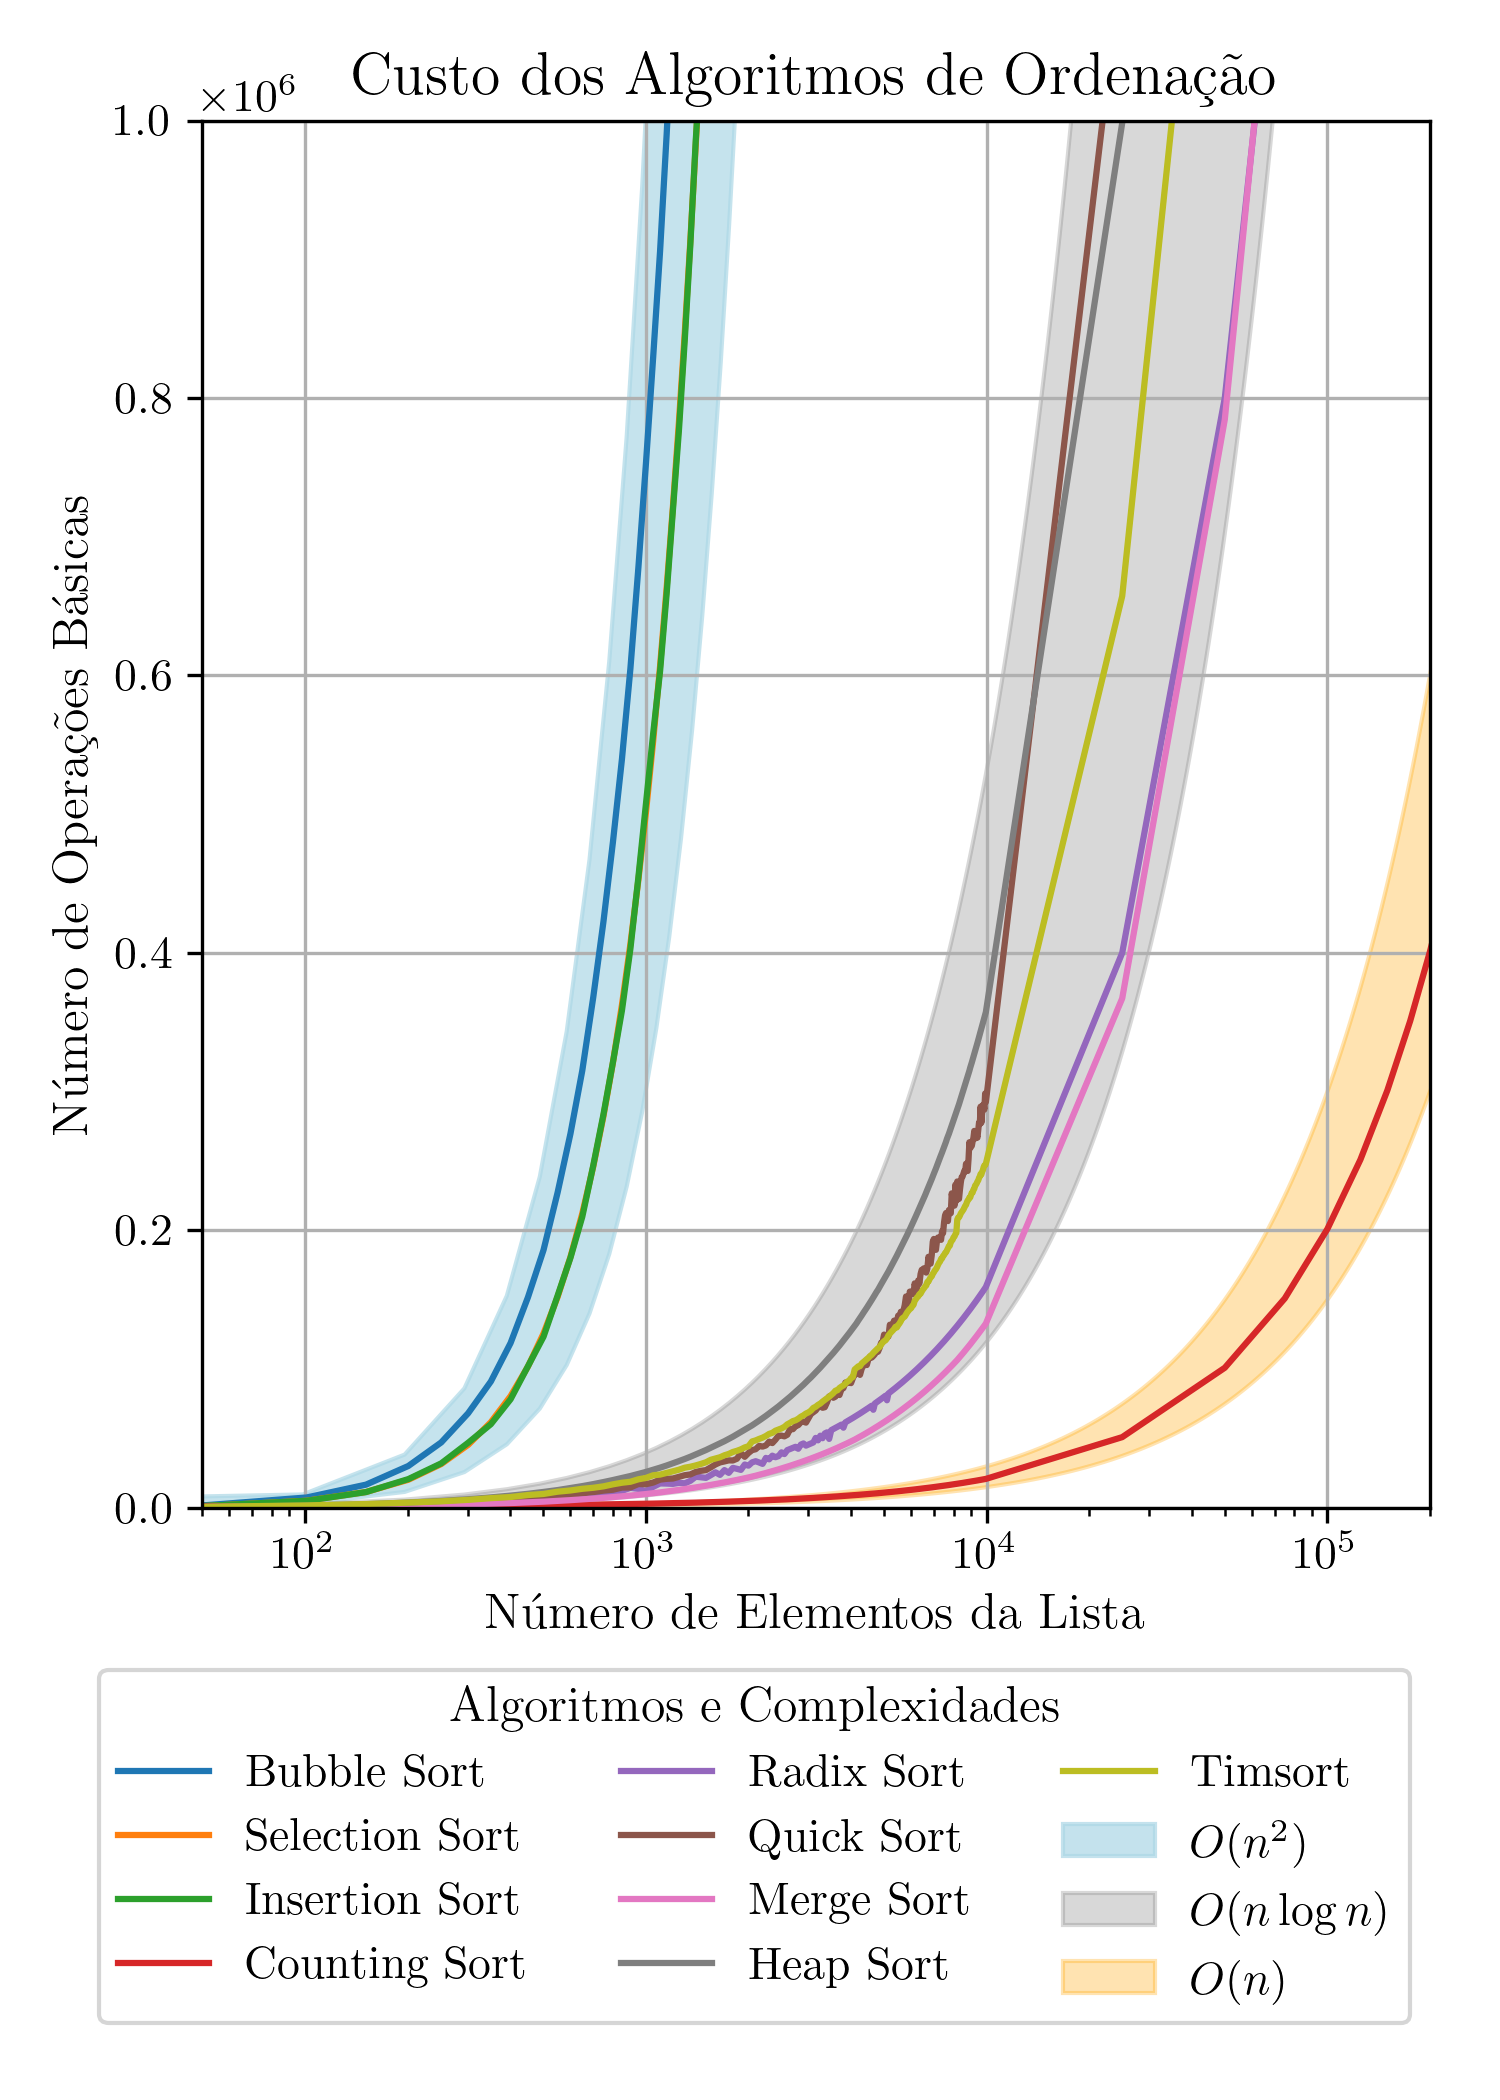
\includegraphics[width=1\linewidth]{sorting_complexities.png}
    \caption{complxidades baseadas no num de ops basicas em listas geradas com numeros inteiros positivos aleatorios até 1000}
    \label{fig:sorting_complexities}
\end{figure}



\bibliographystyle{IEEEtran}
\bibliography{references}

\end{document}



